% GNUPLOT: LaTeX picture with Postscript
\begingroup
  \makeatletter
  \providecommand\color[2][]{%
    \GenericError{(gnuplot) \space\space\space\@spaces}{%
      Package color not loaded in conjunction with
      terminal option `colourtext'%
    }{See the gnuplot documentation for explanation.%
    }{Either use 'blacktext' in gnuplot or load the package
      color.sty in LaTeX.}%
    \renewcommand\color[2][]{}%
  }%
  \providecommand\includegraphics[2][]{%
    \GenericError{(gnuplot) \space\space\space\@spaces}{%
      Package graphicx or graphics not loaded%
    }{See the gnuplot documentation for explanation.%
    }{The gnuplot epslatex terminal needs graphicx.sty or graphics.sty.}%
    \renewcommand\includegraphics[2][]{}%
  }%
  \providecommand\rotatebox[2]{#2}%
  \@ifundefined{ifGPcolor}{%
    \newif\ifGPcolor
    \GPcolortrue
  }{}%
  \@ifundefined{ifGPblacktext}{%
    \newif\ifGPblacktext
    \GPblacktextfalse
  }{}%
  % define a \g@addto@macro without @ in the name:
  \let\gplgaddtomacro\g@addto@macro
  % define empty templates for all commands taking text:
  \gdef\gplbacktext{}%
  \gdef\gplfronttext{}%
  \makeatother
  \ifGPblacktext
    % no textcolor at all
    \def\colorrgb#1{}%
    \def\colorgray#1{}%
  \else
    % gray or color?
    \ifGPcolor
      \def\colorrgb#1{\color[rgb]{#1}}%
      \def\colorgray#1{\color[gray]{#1}}%
      \expandafter\def\csname LTw\endcsname{\color{white}}%
      \expandafter\def\csname LTb\endcsname{\color{black}}%
      \expandafter\def\csname LTa\endcsname{\color{black}}%
      \expandafter\def\csname LT0\endcsname{\color[rgb]{1,0,0}}%
      \expandafter\def\csname LT1\endcsname{\color[rgb]{0,1,0}}%
      \expandafter\def\csname LT2\endcsname{\color[rgb]{0,0,1}}%
      \expandafter\def\csname LT3\endcsname{\color[rgb]{1,0,1}}%
      \expandafter\def\csname LT4\endcsname{\color[rgb]{0,1,1}}%
      \expandafter\def\csname LT5\endcsname{\color[rgb]{1,1,0}}%
      \expandafter\def\csname LT6\endcsname{\color[rgb]{0,0,0}}%
      \expandafter\def\csname LT7\endcsname{\color[rgb]{1,0.3,0}}%
      \expandafter\def\csname LT8\endcsname{\color[rgb]{0.5,0.5,0.5}}%
    \else
      % gray
      \def\colorrgb#1{\color{black}}%
      \def\colorgray#1{\color[gray]{#1}}%
      \expandafter\def\csname LTw\endcsname{\color{white}}%
      \expandafter\def\csname LTb\endcsname{\color{black}}%
      \expandafter\def\csname LTa\endcsname{\color{black}}%
      \expandafter\def\csname LT0\endcsname{\color{black}}%
      \expandafter\def\csname LT1\endcsname{\color{black}}%
      \expandafter\def\csname LT2\endcsname{\color{black}}%
      \expandafter\def\csname LT3\endcsname{\color{black}}%
      \expandafter\def\csname LT4\endcsname{\color{black}}%
      \expandafter\def\csname LT5\endcsname{\color{black}}%
      \expandafter\def\csname LT6\endcsname{\color{black}}%
      \expandafter\def\csname LT7\endcsname{\color{black}}%
      \expandafter\def\csname LT8\endcsname{\color{black}}%
    \fi
  \fi
%  Original size:
%  \setlength{\unitlength}{0.0500bp}%
% Half the original size
  \setlength{\unitlength}{0.0250bp}%
  \begin{picture}(5668.00,3968.00)%
    \gplgaddtomacro\gplbacktext{%
      \csname LTb\endcsname%
      \put(718,704){\makebox(0,0)[r]{\strut{}\scriptsize $10^{-10}$}}%
      \put(718,1030){\makebox(0,0)[r]{\strut{}\scriptsize $10^{-9}$}}%
      \put(718,1355){\makebox(0,0)[r]{\strut{}\scriptsize $10^{-8}$}}%
      \put(718,1681){\makebox(0,0)[r]{\strut{}\scriptsize $10^{-7}$}}%
      \put(718,2006){\makebox(0,0)[r]{\strut{}\scriptsize $10^{-6}$}}%
      \put(718,2332){\makebox(0,0)[r]{\strut{}\scriptsize $10^{-5}$}}%
      \put(718,2657){\makebox(0,0)[r]{\strut{}\scriptsize $10^{-4}$}}%
      \put(718,2983){\makebox(0,0)[r]{\strut{}\scriptsize $10^{-3}$}}%
      \put(718,3308){\makebox(0,0)[r]{\strut{}\scriptsize $10^{-2}$}}%
      \put(850,484){\makebox(0,0){\strut{}\scriptsize $10^{-12}$}}%
      \put(1726,484){\makebox(0,0){\strut{}\scriptsize $10^{-10}$}}%
      \put(2602,484){\makebox(0,0){\strut{}\scriptsize $10^{-8}$}}%
      \put(3478,484){\makebox(0,0){\strut{}\scriptsize $10^{-6}$}}%
      \put(4354,484){\makebox(0,0){\strut{}\scriptsize $10^{-4}$}}%
      \put(5230,484){\makebox(0,0){\strut{}\scriptsize $10^{-2}$}}%
      \put(80,2006){\rotatebox{90}{\makebox(0,0){\strut{}error}}}%
      \put(3259,154){\makebox(0,0){\strut{}Finite difference perturbation}}%
      \put(3259,3638){\makebox(0,0){\strut{}Validation of adjoint gradient wrt. finite differences}}%
    }%
    \gplgaddtomacro\gplfronttext{%
      \csname LTb\endcsname%
      \put(4945,3157){\makebox(0,0)[r]{\strut{}\scriptsize $\Vert\nabla_{FD}-\nabla_{adj}\Vert_2$}}%
    }%
    \gplbacktext
%   Original include, unscaled.
%    \put(0,0){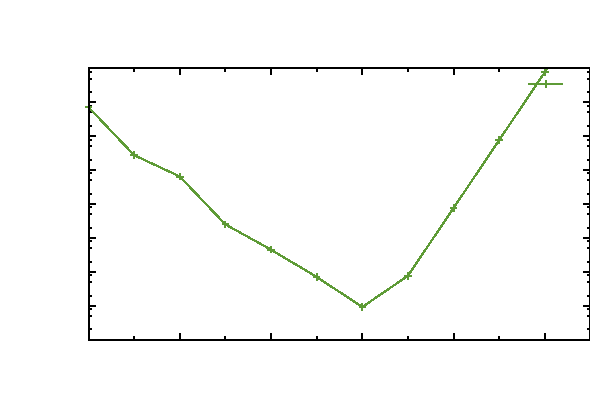
\includegraphics{fdvalidation}}%
%   Scaled-down include
%    \put(0,0){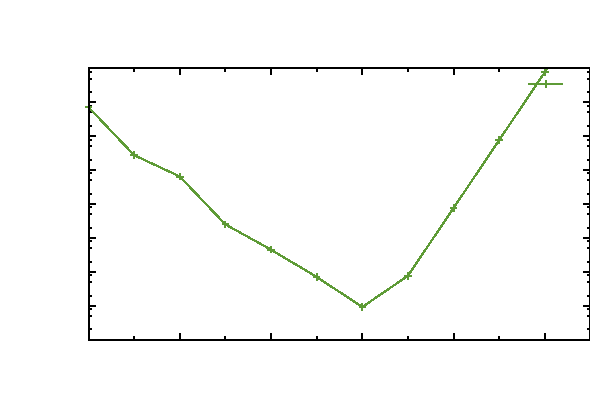
\includegraphics[scale=.5]{fdvalidation}}%
    \gplfronttext
  \end{picture}%
\endgroup
